\documentclass[12pt, letterpaper]{article}
\usepackage{amsmath, amssymb}
\usepackage{geometry}
\usepackage{tikz}
\usepackage{parskip}
\geometry{margin=1in}

\begin{document}

\begin{enumerate}
    \item \textbf{Muhammad Zaky Zein (5025241148) – Halaman 554 Nomor 7}
    \[
    \int_{e}^{+\infty} \frac{1}{x \ln^3 x} \, dx
    \]
    \begin{center}
    \fbox{
        \begin{minipage}{0.25\textwidth}
            \begin{align*}
            \text{Misal:} \quad u &= \ln x \\
                    \frac{du}{dx} &= \frac{1}{x} \\
                               du &= \frac{dx}{x} \\
            \end{align*}
        \end{minipage}
    }   
    \end{center}

    \begin{center}
    \fbox{
        \begin{minipage}{0.55\textwidth}
            \begin{align*}
            \text{Batas baru:} \quad & x = e \Rightarrow u = \ln e = 1 \\
                                     & x = +\infty \Rightarrow u = \ln(+\infty) = +\infty \\
            \end{align*}
        \end{minipage}
    }
    \end{center}
    
    \begin{align*}
    \int_{e}^{+\infty} \frac{1}{x \ln^3 x} \, dx
    &= \int_{e}^{+\infty} \frac{1}{u^3} \, du \\
    &= \int_{1}^{+\infty} u^{-3} \, du \\
    &= \left[ \frac{u^{-2}}{-2} \right]_{1}^{+\infty} \\
    &= \left[ \frac{1}{-2 \cdot u^2} \right]_{1}^{+\infty} \\
    &= 0 - \frac{1}{-2} \\
    &= \frac{1}{2}
    \end{align*}

    \item \textbf{Muhammad Zaky Zein (5025241148) – Halaman 554 Nomor 59} \\
     In electromagnetic theory, the magnetic potential at a point on the axis of a circular coil is given by
    \[
    u = \frac{2 \pi NIr}{k} \int_{a}^{+\infty} \frac{dx}{(r^2 + x^2)^{3/2}}
    \]
    Where $N, I, r, k,$ and $a$ are constants. Find $u$.
    
    Gambar segitiga:
    \begin{center}
    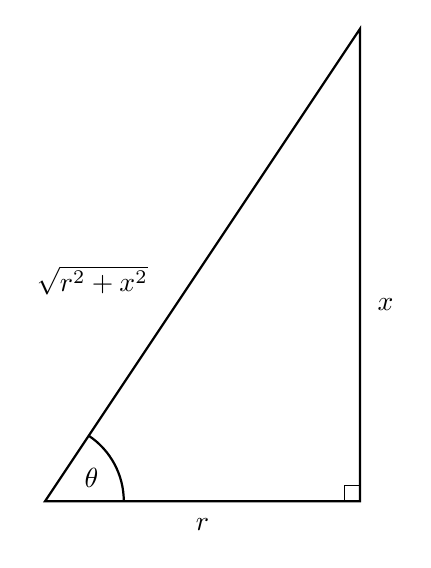
\begin{tikzpicture}[scale=2]
        \draw[thick] (0,0) -- (2,0) -- (2,3) -- cycle;
    
        \draw (2,0) rectangle (1.9,0.1);
        
        \node at (1, -0.05) [below] {$r$};
        \node at (2.05, 1.25) [right] {$x$};
        \node at (0.3, 1.25) [above] {$\sqrt{r^2 + x^2}$};

        \draw[-, thick] (0.5, 0) arc[start angle=0, end angle=56, radius=0.5];
        \node at (0.4, 0.15) [left] {$\theta$};
    \end{tikzpicture}
    \end{center}

    \begin{center}
    \fbox{
        \begin{minipage}{0.3\textwidth}
            \begin{align*}
            \text{Subtitusi:} \quad x &= r \tan \theta \\
                  \frac{dx}{d \theta} &= r \sec^2 \theta \\
                                   dx &= r \sec^2 \theta d \theta \\
            \end{align*}
        \end{minipage}
    }   
    \end{center}

    \[
    \in \frac{dx}{(r^2 + x^2)^{3/2}}
    \]
    
    \begin{align*}
    \int \frac{dx}{(r^2 + x^2)^{3/2}}
    &= \int \frac{r \sec^2 \theta d \theta}{(r^2 + r^2 \tan^2 \theta)^{3/2}} \\
    &= \int \frac{r \sec^2 \theta d \theta}{(r^2(1+ \tan^2 \theta))^{3/2}} \\
    &= \int \frac{r \sec^2 \theta d \theta}{(r^2(\sec^2 \theta))^{3/2}} \\
    &= \int \frac{r \sec^2 \theta d \theta}{r^3 \sec^3 \theta} \\
    &= \int \frac{d \theta}{r^2 \sec \theta} \\
    &= \frac{1}{r^2} \int \cos \theta \, d \theta \\
    &= \frac{1}{r^2} (\sin \theta) + C \\
    &= \frac{x}{r^2 \sqrt{r^2 + x^2}} + C
    \end{align*}

    Hitung Integral tertentu:

    \begin{align*}
    \int_{a}^{+\infty} \frac{dx}{(r^2 + x^2)^{3/2}}
    &= \frac{1}{r^2} \left[ \frac{x}{\sqrt{r^2 + x^2}} \right]_{a}^{+\infty}\\
    &= \frac{1}{r^2} \left[ \left( \frac{x}{x \sqrt{\frac{r^2}{x^2}+1}} \right) \right]_{a}^{+\infty} \\
    &= \frac{1}{r^2}  \left( \frac{1}{\sqrt{1}} - \frac{a}{\sqrt{r^2 + a^2}} \right) \\
    &= \frac{1}{r^2}  \left( 1 - \frac{a}{\sqrt{r^2 + a^2}} \right) \\
    &= \frac{1}{r^2} - \frac{a}{r^2 \sqrt{r^2 + a^2}}
    \end{align*}

    Dapatkan nilai u:

    \begin{align*}
    u &= \frac{2 \pi NIr}{k} \int_{a}^{+\infty} \frac{dx}{(r^2 + x^2)^{3/2}} \\
    &= \frac{2 \pi NIr}{k} \left( \frac{1}{r^2} - \frac{a}{r^2 \sqrt{r^2 + a^2}} \right) \\
    &= \frac{2 \pi NIr}{kr} - \frac{2 \pi N I a}{r \sqrt{r^2 + a^2}}
    \end{align*}
    
\end{enumerate}

\newpage

\begin{enumerate}
    \setcounter{enumi}{2}
    
    \item \textbf{Muhammad Zaky Zein (5025241148) – Halaman 226 Nomor 10}
    \[
    \lim_{t \to 0} \frac{t e^t}{1 - e^t}
    \]
    Substitusi langsung:
    \[
    \frac{0}{0} \quad \text{(Bentuk tak tentu: } \frac{0}{0} \text{)}
    \]
    Gunakan Aturan L’Hôpital:
    \begin{align*}
    \lim_{t \to 0} \frac{\frac{d}{dt}(t e^t)}{\frac{d}{dt}(1 - e^t)} 
    &= \lim_{t \to 0} \frac{e^t + t e^t}{-e^t} \\
    &= \frac{1 + 0}{-1} \\
    &= -1
    \end{align*}

    \item \textbf{Muhammad Zaky Zein (5025241148) – Halaman 226 Nomor 24}
    \[
    \lim_{x \to 0^+} \tan x \cdot \ln x
    \]
    Subtitusi langsung:
    \[
    \lim_{x \to 0^+} \tan x \cdot \ln x = 0 \cdot -\infty \quad \text{(Bentuk tak tentu: } 0 \cdot -\infty \text{)}
    \]
    Ubah bentuk fungsi:
    \[
    \lim_{x \to 0^+} \frac{\ln x}{\cot x}
    \]
    Gunakan Aturan L’Hôpital:
    \begin{align*}
    \lim_{x \to 0^+} \frac{\frac{d}{dx} (\ln x)}{\frac{d}{dx} (\cot x)}
    &=\lim_{x \to 0^+} \frac{\frac{1}{x}}{-\csc^2 x} \\
    &= -\lim_{x \to 0^+} \frac{1}{x \csc^2 x} \\
    &= -\lim_{x \to 0^+} \frac{\sin^2 x}{x} \\
    &= -\lim_{x \to 0^+} \left( \sin x \cdot \frac{\sin x}{x} \right) \\
    &= -\left( \lim_{x \to 0^+} \sin x \cdot \lim_{x \to 0^+} \frac{\sin x}{x} \right) \\
    &= - (0 \cdot 1) \\
    &= 0
    \end{align*}

    \item \textbf{Muhammad Zaky Zein (5025241148) – Page 227 Problem 58} \\
    There is a myth among beginning calculus students that indeterminate forms such as $0^0$, $\infty^0$, and $1^\infty$ always equal 1 because "anything to the zero power is 1" and "1 to any power is 1." The fallacy lies in the fact that these are not actual numbers but rather descriptions of limits. The following examples, suggested by Prof. Jack Staib of Drexel University, show that such indeterminate forms can yield any positive real value:
    
    \begin{enumerate}
        \item 
        \[
        \lim_{x \to 0^+} x^{\frac{\ln a}{1 + \ln x}} = a \quad \text{(form: } 0^0 \text{)}
        \]
    
        \item 
        \[
        \lim_{x \to +\infty} x^{\frac{\ln a}{1 + \ln x}} = a \quad \text{(form: } \infty^0 \text{)}
        \]
    
        \item 
        \[
        \lim_{x \to 0} (x + 1)^{\frac{\ln a}{x}} = a \quad \text{(form: } 1^\infty \text{)}
        \]
    \end{enumerate}
    Verify these results.

    Jawab:
    \begin{enumerate}
        \item 
        \begin{align*}
            \lim_{x \to 0^+} y &= \lim_{x \to 0^+} x^{\frac{\ln a}{1 + \ln x}} \\
        \lim_{x \to 0^+} \ln y &= \lim_{x \to 0^+} \frac{\ln a}{1 + \ln x} \cdot \ln x \\
        \lim_{x \to 0^+} \ln y &= \ln a \cdot \lim_{x \to 0^+} \frac{\ln x}{1 + \ln x}
        \end{align*}
        Evaluasi nilai limit:
        \begin{align*}
        \lim_{x \to 0^+} \frac{\ln x}{1 + \ln x} &= \lim_{x \to 0^+} \frac{1}{\frac{1}{\ln x} + 1} \\
        &= \frac{1}{0+1} \\
        &= 1
        \end{align*}
        Jadi:
        \begin{align*}
        \lim_{x \to 0^+} \ln y &= \ln a \cdot 1 \\
            \lim_{x \to 0^+} y &= a
        \end{align*}
        Terbukti.
        
        \item 
        \begin{align*}
            \lim_{x \to +\infty} y &= \lim_{x \to +\infty} x^{\frac{\ln a}{1 + \ln x}} \\
        \lim_{x \to +\infty} \ln y &= \lim_{x \to +\infty} \frac{\ln a}{1 + \ln x} \cdot \ln x \\
        \lim_{x \to +\infty} \ln y &= \ln a \cdot \lim_{x \to +\infty} \frac{\ln x}{1 + \ln x}
        \end{align*}
        Evaluasi nilai limit:
        \begin{align*}
        \lim_{x \to +\infty} \frac{\ln x}{1 + \ln x} &= \lim_{x \to +\infty} \frac{1}{\frac{1}{\ln x} + 1} \\
        &= \frac{1}{0+1} \\
        &= 1
        \end{align*}
        Jadi:
        \begin{align*}
        \lim_{x \to 0^+} \ln y &= \ln a \cdot 1 \\
            \lim_{x \to 0^+} y &= a
        \end{align*}
        Terbukti.
    
        \item 
        \begin{align*}
            \lim_{x \to 0} y &= \lim_{x \to 0} (x + 1)^{\frac{\ln a}{x}} \\
        \lim_{x \to 0} \ln y &= \lim_{x \to 0} \frac{\ln a}{x} \cdot \ln (x + 1) \\
        \lim_{x \to 0} \ln y &= \ln a \cdot \lim_{x \to 0} \frac{\ln (x+1)}{x} \\
        \end{align*}
        Evaluasi nilai limit dengan menggunakan aturan L’Hôpital:
        \begin{align*}
        \lim_{x \to 0} \frac{\ln (x+1)}{x}
        &= \lim_{x \to 0} \frac{\frac{d}{dx} (\ln (x+1))}{\frac{d}{dx}(x)} \\
        &= \lim_{x \to 0} \frac{\frac{1}{x +1}}{1} \\
        &= \frac{\frac{1}{1}}{1} \\
        &= 1
        \end{align*}
        Jadi:
        \begin{align*}
        \lim_{x \to 0} \ln y &= \ln a \cdot 1 \\
            \lim_{x \to 0} y &= a
        \end{align*}
        Terbukti.
        
    \end{enumerate}
    
\end{enumerate}

\end{document}